%% Total contracts = 65
%% Total checks = 52988839
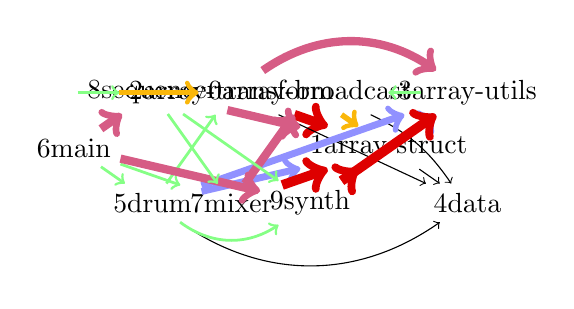
\begin{tikzpicture}

  \node (00)               {\rkt{3}{array-utils}};
  \node (01) [below of=00,yshift=0.3cm] {};
  \node (02) [below of=01,yshift=0.3cm] {\rkt{4}{data}};

  \node (10) [left of=00] {};
  \node (11) [left of=01] {\rkt{1}{array-struct}};
  \node (12) [left of=02] {};

  \node (20) [left of=10] {\rkt{0}{array-broadcast}};
  \node (21) [left of=11] {};
  \node (22) [left of=12] {\rkt{9}{synth}};

  \node (30) [left of=20] {\rkt{2}{array-transform}};
  \node (31) [left of=21] {};
  \node (32) [left of=22] {\rkt{7}{mixer}};

  \node (40) [left of=30] {\rkt{8}{sequencer}};
  \node (41) [left of=31] {};
  \node (42) [left of=32] {\rkt{5}{drum}};

  \node (51) [left of=41] {\rkt{6}{main}};

  %% -- edges
  %% array broadcast
  \draw[->,yellow!45!orange, line width=2pt] (20) -- (11);
  \draw[->,green!48!white, line width=1pt] (20) -- (00);
%% WARNING: no data for boundary 'data.rkt' ==> 'array-broadcast.rkt'
  \draw[->] (20) edge[bend left=15] (02);
  %% array-struct
  \draw[->,blue!43!white, line width=2.5pt] (11) -- (00);
%% WARNING: no data for boundary 'data.rkt' ==> 'array-struct.rkt'
  \draw[->] (11) -- (02);
  %% array-transform
  \draw[->,yellow!45!orange, line width=2pt] (30) -- (20);
  \draw[->,red!87!black, line width=3.5pt] (30) -- (11);
  \draw[->,purple!64!white, line width=3pt] (30) edge[bend left=35] (00);
%% WARNING: no data for boundary 'data.rkt' ==> 'array-transform.rkt'
  \draw[->] (30) -- (02);
  %% drum
  \draw[->,blue!43!white, line width=2.5pt] (42) -- (11);
  \draw[->,green!48!white, line width=1pt] (42) -- (30);
  \draw[->,blue!43!white, line width=2.5pt] (42) -- (00);
%% WARNING: no data for boundary 'data.rkt' ==> 'drum.rkt'
  \draw[->] (42) edge[bend right=35] (02);
  \draw[->,green!48!white, line width=1pt] (42) edge[bend right=35] (22);
  %% main
  \draw[->,green!48!white, line width=1pt] (51) -- (42);
  \draw[->,green!48!white, line width=1pt] (51) -- (32);
  \draw[->,purple!64!white, line width=3pt] (51) -- (40);
  \draw[->,purple!64!white, line width=3pt] (51) -- (22);
  %% mixer
  \draw[->,purple!64!white, line width=3pt] (32) -- (20);
  \draw[->,red!87!black, line width=3.5pt] (32) -- (11);
  %% sequencer
  \draw[->,purple!64!white, line width=3pt] (40) -- (11);
  \draw[->,green!48!white, line width=1pt] (40) -- (30);
  \draw[->,green!48!white, line width=1pt] (40) -- (32);
  \draw[->,green!48!white, line width=1pt] (40) -- (22);
  %% synth
  \draw[->,red!87!black, line width=3.5pt] (22) -- (11);
  \draw[->,red!87!black, line width=3.5pt] (22) -- (00);

\end{tikzpicture}
